\documentclass{article}


% This file is a solution template for:
% 1 inch margins
\usepackage{fullpage}

\usepackage{hyperref}
\usepackage{graphicx}
\usepackage{multicol}
\usepackage{subcaption}

% Add ability to resume enumeration environments with /begin{enumerate}[resume]
\usepackage{enumitem}

\usepackage{pgf}
\usepackage{tikz}
\usepackage{bodegraph}
\usepackage{circuitikz}
\usetikzlibrary{calc}
\usetikzlibrary{trees}
\usetikzlibrary{arrows}
\usetikzlibrary{shapes}
\usetikzlibrary{fadings}
\usetikzlibrary{positioning}
\usetikzlibrary{intersections}

\usepackage[english]{babel}
\usepackage[latin1]{inputenc}
\usepackage[T1]{fontenc}
% Or whatever. Note that the encoding and the font should match. If T1 does not look nice, try deleting the line with the fontenc.


\usepackage{listings}

\usepackage{amsmath}


\usepackage{xspace}
\newcommand{\Ohm}{$\Omega$\xspace}

% No author or date
\author{}
\date{}




\title{Bipolar Junction Transistors}


\begin{document}
\maketitle

\section{Introduction}
This week we introduce the transistor.  Transistors are three-terminal devices that can amplify a signal and increase the signal's power. The price is that we must also supply DC power to it (hence, the need for three terminals).  Figure~\ref{fig:transistor-TO-92} shows a classic transistor package style.

\begin{figure}
\begin{center}
\begin{subfigure}{0.4\textwidth}
\begin{center}
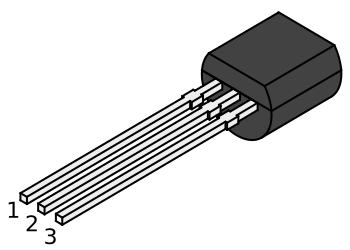
\includegraphics[width=0.8\textwidth]{pics/TO-92_Front_with_Pin_Numbers}
\end{center}
\caption{front view}
\end{subfigure}
\begin{subfigure}{0.4\textwidth}
\begin{center}
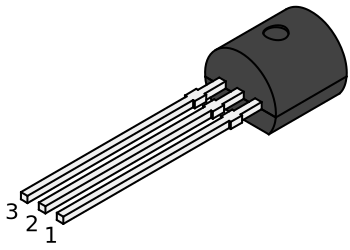
\includegraphics[width=0.8\textwidth]{pics/TO-92_Back_with_Pin_Numbers}
\end{center}
\caption{back view}
\end{subfigure}
\end{center}
\caption{Transistors in the 2N series are commonly found in the industry-standard TO-92 package with emitter on pin 1, base on pin 2, and collector on pin 3.}
\label{fig:transistor-TO-92}
\end{figure}

The three terminals are called the emitter, the base and the collector. The base is the control terminal -- a small current enters here and controls the big current that flows from collector to emitter. The notation may seem odd, but remember that electrons actually carry most currents and they have negative charge. A positive current flowing from the collector to the emitter means that electrons are flowing from the emitter to the collector.

In this chapter we will use a simple model for this device to try to understand its rather complicated behavior. As we continue through the semester we will encounter additional devices that require some sort of approximate models to describe their expected behavior. Since there are always approximations to the real devices they will have certain shortcomings or conditions were the models no longer apply. 

\subsection{The Basic Transistor Model}
Bipolar transistors are essentially two diodes placed back to back. This may seem like a silly thing to do but the diodes are not the same. When current flows through one diode it provides carriers to carry current through the other part of the element. Thus, in its most basic form, a transistor is a current amplifier.

Bipolar transistors come in two basic types: npn and pnp. The current flow in a npn transistor shown schematically in Figure~\ref{fig:transistors_with_currents}. Current (conventionally defined as the movement of positive charges) goes in through the base terminal and out the emitter and the amplified current flows from the collector to the emitter. 

\begin{figure}
\begin{center}
\begin{subfigure}{0.4\textwidth}
\begin{center}
\includegraphics[width=0.7\textwidth]{pics/npn_transistor_with_currents}
\end{center}
\caption{npn transistor}
\end{subfigure}
\begin{subfigure}{0.4\textwidth}
\begin{center}
\includegraphics[width=0.7\textwidth]{pics/pnp_transistor_with_currents}
\end{center}
\caption{pnp transistor}
\end{subfigure}
\end{center}
\caption{During standard operation of npn and pnp bipolar junction transistors the collector-emitter current $I_{ce}$ will be $\beta$ times larger than the base-emitter current $I_{be}$.}
\label{fig:transistors_with_currents}
\end{figure}

Our first model of the transistor says that the collector-emitter current, $I_{ce}$, is $\beta$ times the base-emitter current, $I_{be}$. Later, we will see that good designs do not depend on $\beta$ since it varies from one device to the next, and it depends on the operating conditions (e.g. temperature). Most transistors have a value of $\beta \approx 100$. In this week's laboratory, you will measure $\beta$ for a 2N3904 transistor. 

In an npn transistor, a current will flow from the base to the emitter only if the base voltage is positive with respect to the emitter. A collector current will flow to the emitter only if the collector is positive with respect to the emitter. In a pnp transistor, things are reversed, and a current will flow from the emitter to the base only if the base voltage is negative with respect to the emitter. A collector current will flow from the emitter only if the collector is negative with respect to the emitter. The arrow on the emitter tells you which way the current is supposed to flow, and which also indicates whether the base voltage must be positive or negative with respect to the collector.

Let's summarize the conditions required for an npn transistor to conduct (the ``transistor rules''):
\begin{enumerate}
\item $V_{be} > 0$.  Since this is a diode, $V_{be}$ should be roughly 0.6\,V when it is conducting.
\item V$_{bc} < 0$. This is a reverse-biased diode with enough voltage that the base current normally flows to the emitter. You do not want current to flow from the base to the collector (i.e. $V_{bc} > 0$).
\item $I_{ce} = \beta I_{be}$.
\end{enumerate}

Under normal operating conditions we will have a resistor (or load) connected to the emitter or to the collector, and we will see a voltage drop across the load as $I_{ce}$ flows through the transistor. If $I_{ce}$ changes it will change the voltage drop across the transistor ($V_{ce}$). If $V_{ce}$ drops too low, then $V_{bc}$ will become positive since $V_{be}$ must still be roughly 0.6\,V. Current then flows from the base to the collector, leading to an apparent drop in $\beta$. This is called saturation.

\section{Basic Transistor Circuits}
Here are some basic circuits which illustrate the operation of transistors.

\subsection{Constant Current Source}
The current source is the simplest transistor circuit possible and is shown in Figure~\ref{fig:npn_current_source}. You simply drive a small current, $I_{be}$, into the base of a transistor, and it produces a large current, $I_{ce}$, through the rest of the circuit. In this case $I_{be}$ is given by,
\begin{equation}
V_+ - V_{be} = I_{be} R_b
\end{equation}
and the current through the load can then be calculated from our current gain model ($I_{ce} = \beta I_{be}$). From this we can see that current flowing through the load does not depend on the load resistance. It does depend on $\beta$ so it is not an ideal design.

\begin{figure}
\begin{center}
\begin{tikzpicture}
\draw (1.5,1) node[npn](npn){};
\draw (1.5,0) node[ground]{} to (npn.E);
\draw (npn.C) to[vR,l=$R_L$] (1.5,3) to[short,-o] (1.5,3.5) node[above]{$V_{cc}$};
\draw (-1,1) node[left]{$V_+$} to[R,o-,l=$R_b$] (npn.B);
\end{tikzpicture}
\end{center}
\caption{A basic npn transistor current source.}
\label{fig:npn_current_source}
\end{figure}

The current flowing through the load should be independent of the load resistance. If your load resistor gets too big, though, the voltage drop across the load will make $V_{cb}$ too small to conduct. In this case the current $I_{ce}$ will drop until the transistor starts to conduct again. This reduces the effective $\beta$ of the transistor (i.e. some base current flows to the collector). This condition is called \emph{saturation}.

\subsection{Transistor Switch}
We can use a transistor switch to control a big current with a small current. This is just a current source with the device you wish to switch in place of the load resistor. A common application is to use a digital (0 or 5\,V) signal with moderate impedance to control a device requiring a lot more power. Using this circuit we could use the 5\,V TTL (transistor-transistor logic) output of a function generator in the lab to drive a light bulb.

In designing a transistor switch you want most of the voltage drop to be across your device. If $V_{ce}$ is large then the power dissipated inside the transistor ($I_{ce} V_{ce}$) will destroy the transistor. You can get around this in your design by designing the switch for saturated operation. Since the switch runs in saturation mode, some of the base current will flow up to the collector and the apparent $\beta$ will be smaller than our nominal 100. A common design strategy is to design for a ``generous base current,'' which could be satisfied with an effective gain of roughly 10. 

\subsection{The Emitter-Follower Amplifier}
One of the most important circuits in this chapter is the emitter-follower (see Figure~\ref{fig:emitter_follower}). This is a very easy circuit to design, and its normal operating conditions do not depend on $\beta$. An input voltage on the base produces a base current and an amplified collector current, to generate a voltage drop across the emitter resistor. But the voltage of the emitter cannot increase beyond $v_{in} - 0.6$\,V, or the base current will drop. Consequently, the circuit produces a voltage of $v_{in} - 0.6$\,V at the output. In other words, the output (at the emitter) follows the input! In fact, this simple rule, $V_{be} = 0.6$\,V, is usually sufficient to understand most transistor circuits.

\begin{figure}
\begin{center}
\begin{tikzpicture}
\draw (1,2.5) node[npn](npn){};
\draw (npn.E) to[R,l=$R_e$] ++(0,-1.5) node[ground]{};
\draw (npn.C) to[short,-o] ++(0,0.5) node[above]{$V_{cc}$};
\draw (npn.B) to[short,-o] ++(-0.5,0) node[left]{$v_{in}$};
\draw (npn.E) to[short,*-o] ++(1,0) node[right]{$v_{out}$};
\end{tikzpicture}
\end{center}
\caption{The classic emitter-follower amplifier circuit.}
\label{fig:emitter_follower}
\end{figure}

The emitter follower is extremely useful because it transforms impedance. The current amplification of the transistor means that it can drive a low impedance, while pulling only a small current from the source. This is just like the transformer -- but without the transformer's voltage decrease.

In the lab, you will build an emitter follower and measure its impedance. You should find 
\begin{equation}
\frac{Z_{out}}{Z_{source}} = \frac{1}{1 + \beta}
\end{equation}
The derivation of this formula is left to the reader.

\subsection{An Inverting Amplifier}
The final circuit is the inverting amplifier, which is also called a common collector, and is shown in Figure~\ref{fig:inverting_amplifier}. An inverting amplifier is similar to an emitter-follower with two changes. It has an additional resistor between the power supply and the collector, and the output is at the collector terminal. Of course our transistor rules still force the emitter to be $v_{in} - 0.6$\,V, and this will set the transistor current to be 
\begin{equation}
\frac{v_{in} - 0.6\,\mbox{V}}{R_e}.
\end{equation}
When this current passes through the collector resistor, it will generate a voltage drop of 
\begin{equation}
R_c \frac{v_{in} - 0.6\,\mbox{V}}{R_e}.
\end{equation}
which means that the voltage drop across the collector resistor will be approximately $-\frac{R_c}{R_e}$ times the input voltage. The output is then given by
\begin{equation}
v_{out} = V_{cc} - \frac{R_c}{R_e} (v_{in} - 0.6\,\mbox{V}).
\end{equation}

\begin{figure}
\begin{center}
\begin{tikzpicture}
\draw (1,2.5) node[npn](npn){};
\draw (npn.E) to[R,l=$R_e$] ++(0,-1.5) node[ground]{};
\draw (npn.C) to[R,l=$R_c$,-o] ++(0,2) node[above]{$V_{cc}$};
\draw (npn.B) to[short,*-o] ++(-0.5,0) node[left]{$v_{in}$};
\draw (npn.C) to[short,-o] ++(1,0) node[right]{$v_{out}$};
\end{tikzpicture}
\end{center}
\caption{An npn transistor inverting amplifier.}
\label{fig:inverting_amplifier}
\end{figure}

The minus sign means that when the voltage at the base is zero, the collector will read the full supply voltage. When the voltage at the base is high there will be a big current and the collector voltage will drop almost to zero. Thus the output will be exactly the opposite of the input. If you find this disturbing you can use two inverting amplifiers in series to get a non-inverting amplifier.

\section{AC Transistor Amplifiers}
The simple transistor amplifiers that we studied in the previous section have some serious problems for use in AC signals. Their most serious shortcoming is that there is a ``dead region'' where small signals do not turn on the transistor. So, if your signal is smaller than 0.6\,V, or if it is negative, the transistor does not conduct and the amplifier does not work. 

\subsection{Design goals for an AC amplifier}
Before moving on to making a better AC amplifier, let's define some useful terms. We define the \emph{output range} to be the range of possible output voltages. We refer to the maximum and minimum output voltages as the \emph{rail voltages} and the \emph{output swing} is the difference between the rail voltages. The input range is the range of input voltages that produce outputs which are not at either rail voltage. 
Our goal in designing an AC amplifier is to get an input range and output range which is symmetric around zero and  that there is not a dead region. To do this we need make sure that the transistor is in conduction for all of our input range. How does this work? We do it by adding an offset voltage to the input to make sure the voltage presented to the transistor's base with no input signal, the resting or \emph{quiescent voltage}, is well above ground. In lab 6, the function generator provided the offset, in this chapter we will show how to design an amplifier which provides its own offset.

Now that you understand capacitors it is pretty easy to see how to add and subtract an offset voltage to a signal, at least for AC signals. From here on, you will design transistor circuits with a bias network. This bias network is simply a voltage divider that is connected to the input. Its job is to insure that the output stays at approximately half the supply voltage for small input signals. Then, the output voltage can vary over a wide range (positive and negative) while always keeping the transistor conducting.

The trick to make this work is to separate these quiescent voltages and currents from the input and output signals. To do this, you will use blocking capacitors to isolate the input and the output. If you connect an AC input to a capacitor, it will not pass any DC offset voltages but it does pass the fast AC signals. Similarly, an output blocking capacitor will pass the fast signal while keeping the quiescent (resting) voltage from the amplifier from disturbing whatever comes next. This is shown schematically in the next sections (see for example Figure~\ref{fig:AC_emitter_follower}).

\subsection{Some Design Basics}
This week we are going to redesign our emitter follower and inverting amplifier to use bias networks. To help you with your design, we will make a step by step list for designing each of these basic transistor circuits. 

Here are a couple initial design decisions we will make:
\begin{itemize}
\item You will begin by determining the quiescent (DC, no signal) current through the collector. You usually want the quiescent current to be larger than any current you will use to drive a load. A quiescent current of 1\,mA is typical, and we will use that in our example designs. 
\item We will also use a single +15\,V power supply to power the collector (the common collector voltage or $V_{cc}$) for and the bias network.
\item We need to be careful about loading the different stages of this amplifier.  The transistor's base current will load the output of our bias voltage divider. To bias the base, we need a stiff voltage divider (i.e. low impedance). Our rule of thumb for designing voltage dividers was to have a factor of 10 difference in impedance at each stage. 
\end{itemize}

\begin{figure}
 \begin{center}
  \begin{circuitikz}
   \draw (4,4) node[npn](npn){} node{};
   \draw (npn.B) to[short] ++(-1,0) node[circ](div){} to[C,l=$C_{in}$,-o] ++(-1.5,0) node[anchor=east]{$v_{in}$};
   \draw (npn.C) to[short] ++(0,2) node[circ](vcc){} to[short,-o] ++(0,0.5) node[anchor=south]{$V_{cc}$};
   \draw (npn.E) to[C,l=$C_{out}$,*-o] ++(1.5,0) node[anchor=west]{$v_{out}$};
   \draw (npn.E) to[R,l=$R_e$,-*] ++(0,-2.5) node[ground](gnd){};
   \draw (div) to[R,l=$R_1$] ++(0,+2.5) |- (vcc);
   \draw (div) to[R,l=$R_2$] ++(0,-2.5) |- (gnd);
  \end{circuitikz}
 \end{center}
\caption{A biased emitter-follower npn transistor amplifier.}
\label{fig:AC_emitter_follower}
\end{figure}

\subsection{AC Emitter-Follower}
Design steps for the emitter-follower of Figure~\ref{fig:AC_emitter_follower} proceed as follows:
\begin{enumerate}
\item To have the maximum symmetric range of output voltages we would like our quiescent base voltage to be half of the (15\,V) supply voltage. So, we will use a 1:1 input voltage divider. This means that both biasing resistors will be the same.
\item We then choose the emitter resistor. The quiescent voltage at the emitter is a diode drop below the voltage in the middle of the bias network (i.e. $V_{cc}/2$ if we have a 1:1 divider). This is roughly +7\,V in our case. To get our design quiescent current, the emitter resistor must be 
\begin{equation}
R_e = \frac{V_e}{I_e} = \frac{7\,\mbox{V}}{1\,\mbox{mA}} = 7\,\mbox{k}\Omega.
\end{equation}
We will use the standard 6.8\,K\Ohm.  It is close enough.
\item To bias the base we want a stiff voltage divider (i.e. low impedance), therefore we want to use resistors that are smaller than the base-emitter-ground impedance ($Z_b = V_b/I_b \approx 750$\,k\Ohm) by a factor of 10 or so. For this example, we will choose two 75\,k\Ohm resistors for this divider.
\item Remember to AC couple (via capacitors) the input and output. The exact values are not particularly important, though you should remember that you are making a biased high-pass RC filter. Values around 0.1\,$\mu$F are typical if you want $f_{3dB} \approx 20$\,Hz, but you can use what you have as long as it is not too small. 
\end{enumerate}


\begin{figure}
 \begin{center}
  \begin{circuitikz}
   \draw (4,4) node[npn](npn){};
   \draw (npn.B) to[short] ++(-1,0) node[circ](div){} to[C,l=$C_{in}$,-o] ++(-1.5,0) node[anchor=east]{$v_{in}$};
   \draw (npn.E) to[R,l=$R_e$,-*] ++(0,-2) node[ground](gnd){};
   \draw (npn.C) to[R,l=$R_c$] ++(0,2.5) node[circ](vcc){} to[short,-o] ++(0,0.5) node[anchor=south]{$V_{cc}$};
   \draw (npn.C) to[C,l=$C_{out}$,*-o] ++(1.5,0) node[anchor=west]{$v_{out}$};
   \draw (div) to[R,l=$R_1$] ++(0,+2.5) |- (vcc);
   \draw (div) to[R,l=$R_2$] ++(0,-2.5) |- (gnd);
  \end{circuitikz}
 \end{center}
\caption{A biased npn transistor inverting amplifier.}
\label{fig:AC_inverting_amplifier}
\end{figure}

\subsection{Common-Emitter (Inverting) Amplifier}
In this circuit, we need to know the quiescent current and the desired gain. Let's assume a gain of -5 and a 1\,mA quiescent current for this example. The circuit diagram is shown in Figure~\ref{fig:AC_inverting_amplifier}.

\begin{enumerate}
\item In this circuit we want the quiescent output (at the collector) to be set roughly halfway between the power supply and the ground for maximum output voltage swing. For $I_c = 1$\,mA, 
\begin{equation}
R_c = \frac{V_{cc} - V_c}{I_c} \approx \frac{7\,\mbox{V}}{1\,\mbox{mA}} = 7\,\mbox{k}\Omega.
\end{equation}
We will use a standard resistor of about this value (e.g. $R_c = 6.8$\,k\Ohm) as we did for the follower.
\item The emitter resistor can be determined by the desired gain. Previously we saw that 
\begin{equation}
G = -\frac{R_c}{R_e}
\end{equation}
In our case we want a gain of 5 so we chose $R_e = 1.35$\,k\Ohm. We will approximate this by a standard 1.5\,k\Ohm resistor. Note that with this choice, the emitter quiescent voltage will be given by the voltage drop across the emitter resistor $I_c R_e = 1.5$\,V.
\item The tricky part is to design the bias network for this circuit. Since we know the emitter voltage, the output of the bias network (i.e. the base voltage) is just a diode drop higher than the emitter voltage. Therefore the bias resistors must be set to give a base voltage, $V_b$, of 
\begin{equation}
V_b = V_2 = V_e + 0.6\,\mbox{V} = 1.5\,\mbox{V} + 0.6\,\mbox{V} = 2.1\,\mbox{V}.
\end{equation}
This is the drop across the lower of the two bias resistors. The other has a drop of 
\begin{equation}
V_1 = V_{cc} - V_2 = 15\,\mbox{V} - 2.1\,\mbox{V} = 12.9\,\mbox{V}
\end{equation}
The bias network's output impedance must be small enough to keep this bias up even when loaded.  We will select the bias resistors so that the current running through the bias network is about 10 times larger than the current that goes into the base. If $\beta = 100$, then the base current is
\begin{equation}
I_b = \frac{I_c}{\beta} = 10\,\mu\mbox{A},
\end{equation}
and the bias current, $I_{bias}$, is ten times larger: $I_{bias} = 100\,\mu$A. The total resistance of the bias network is $R_1 + R_2$, so we need $R_1 + R_2 = 15\,\mbox{V} / 100\,\mu\mbox{A} = 150$\,k\Ohm.

We can now determine the value for $R_2$, since from the voltage divider formula, we require:
\begin{equation}
\frac{V_b}{V_{cc}} = \frac{R_2}{R_1 + R_2} \Rightarrow R_2 = \frac{2.1\,\mbox{V}}{15\,\mbox{V}} 150\,\mbox{k}\Omega = 21\,\mbox{k}\Omega,
\end{equation}
and therefore, $R_1 = 150\,\mbox{k}\Omega - 21\,\mbox{k}\Omega = 129\,\mbox{k}\Omega$.
\item Remember to AC couple the input and output with capacitors. The values are not particularly important, but the relevant $RC$ time constants should be chosen so as to guarantee unimpeded passage of the AC signal to be amplified.
\end{enumerate}


\pagebreak

\section{Design Exercises}

\begin{enumerate}
\item \label{ex:constant_current_source} Design a npn transistor current source with a base supply voltage of 5\,V, a collector supply voltage of 10\,V, and a target constant current of 1\,mA. Assuming that $\beta = 200$, determine the value of the base resistor, and the range of collector/load resistance over which you expect the current source to produce 1\,mA. What happens when the collector/load resistance goes above this range? 

% \item \label{ex:constant_current_source_saturation} Design a npn transistor switch for a light bulb with a resistance of 50\,\Ohm and a collector supply voltage of 6\,V. Make sure the current into the base will guarantee operation in saturation mode (gain of roughly 10, instead of $\beta = 200$) which is roughly independent of the exact light bulb resistance.

\item \label{ex:emitter_follower} Consider an npn emitter-follower amplifier that has $R_e = 8$\,\Ohm. Calculate the input impedance for the amplifier. Assume that your input signal has a DC bias of 2\,V, and an AC amplitude of 1\,V, and that $\beta = 200$. Determine the collector supply voltage necessary to keep the average power dissipated in the transistor to below 0.5\,W. What is the power dissipated in the 8\,\Ohm load resistor?

% \item \label{ex:AC_emitter_follower} Design an AC emitter-follower with a 1.5\,mA quiescent current. Assume that $V_{cc} = 15$\,V. You can approximate the resistor values by picking the nearest standard values. Show any approximations when they are employed.

\item \label{ex:AC_inverting_amplifier} Design an AC inverting amplifier which should operate at frequencies above 100\,Hz with a 0.2\,mA quiescent current and a gain of 15. Assume that $V_{cc} = 15$\,V, $\beta = 100$, and $R_L = 1$\,M\Ohm.
\end{enumerate}

\section{Lab: Bipolar Junction Transistors and Applications}

\begin{enumerate}
\item (Estimated time: 1 hour) Measure the current gain of a 2N3904 transistor using the constant current source circuit from design exercise~\ref{ex:constant_current_source}. If you measure the collector current through the collector/load resistor for a variety of base currents (i.e. change the base resistor or the voltage applied to it), then you should be able to extract a value for $\beta$. Since $\beta$ value depends on the collector current value, make sure that collector current does not exceed 5\,mA.

% \item (Estimated time: 1 hour) With the component values you calculated for design exercise~\ref{ex:emitter_follower} (appropriately updated for your measured value of $\beta$), verify that the circuit is indeed a constant current source by trying different collector/load resistors and measuring the collector current. Verify that the constant current source goes into saturation when you expect it to.

\item (Estimated time: 1 hour) Construct an emitter-follower amplifier using the 2N3904 (npn) transistor whose gain you have previously measured. The circuit should be based on your calculations for design exercise~\ref{ex:emitter_follower} (adjusted for the actual value of $\beta$ if necessary).
\begin{enumerate}
\item Adjust the function generator to output an AC signal at 1\,kHz with an amplitude of 1\,V and a DC bias of 2\,V.
\item Measure the input impedance of the speaker on your breadboard, and measure the relevant voltages across it when it is attached directly to the function generator.
\item Use the speaker as the load resistor in your emitter-follower circuit, and adjust the collector supply voltage so as to keep the transistor power dissipation below 0.5\,W.
\item Power up your emitter-follower circuit and measure the relevant voltages across the speaker and at the transistor base. Is the speaker louder?
\item Does the output signal sent to the speaker show any signs of distortion? How low can you set the collector voltage before performance is significantly affected? How do you measure the amount of distortion?
\end{enumerate}

% \item Transistor Switch (30 minutes\ldots 1 hour) Construct a voltage controlled transistor switch by connecting the collector of a 2N3904 transistor though a light bulb to a 6\,V power supply (see design exercise~\ref{ex:constant_current_source_saturation). Use a square wave voltage to control the switch. Measure the voltage across the light bulb and compare with your quantitative and qualitative results from a previous lab exercise (if necessary repeat the previous lab exercise).

\item (2 hours\ldots much longer if not prepared) Design and construct a DC-biased common-emitter AC amplifier with a quiescent current of 0.2\,mA, and a gain of $\sim 15$ at 2\,kHz, powered by a +15\,V power supply.  The circuit should be based on your calculations for design exercise~\ref{ex:AC_inverting_amplifier}.
\begin{enumerate}
\item Measure the small-signal AC gain, and compare it to your calculation. Measure the voltage swing (i.e. the maximum output voltage swing before distortion). Measure the output impedance (Suggestion: use AC coupling).
\item Now try to eliminate the emitter resistor without affecting the DC bias, by using a by-pass capacitor parallel to the emitter resistor. Measure the new small-signal gain. Measure and describe any distortion.
\item (Bonus) Short your emitter resistor to obtain the maximum gain. Measure the new small-signal gain. It will be necessary to change your bias network. Does this agree with your expectations? Measure the new voltage swing. Measure and describe any distortion. 
\end{enumerate}

\end{enumerate}


\end{document}
